
%(BEGIN_QUESTION)
% Copyright 2006, Tony R. Kuphaldt, released under the Creative Commons Attribution License (v 1.0)
% This means you may do almost anything with this work of mine, so long as you give me proper credit

Many valve positioner mechanisms use a mechanical component called a {\it cam} to transfer valve stem motion to another form of motion inside the positioner mechanism.  Explain what a ``cam'' is in the general sense, and then identify where one might be used inside a positioner.

To help you in your explanation, examine this illustration of a cam and roller-follower:

$$\includegraphics[width=15.5cm]{i01366x01.eps}$$

\vskip 20pt \vbox{\hrule \hbox{\strut \vrule{} {\bf Suggestions for Socratic discussion} \vrule} \hrule}

\begin{itemize}
\item{} One of the unique benefits of using a cam in a valve positioner is the ability to swap out the cam for one of a different {\it shape}.  Explain what a change in cam shape could do to the behavior of a control valve.
\end{itemize}

\underbar{file i01366}
%(END_QUESTION)





%(BEGIN_ANSWER)

A {\it cam} is a rotating object with an irregular radius, which may be shaped in any way desired to produce a specific relationship between angular displacement and linear displacement:
 
$$\includegraphics[width=15.5cm]{i01366x02.eps}$$

%(END_ANSWER)





%(BEGIN_NOTES)

Some sliding-stem valve positioners use levers to translate linear stem motion into rotary motion, which is then converted back into linear motion through a cam inside the positioner.  Nearly {\it all} rotary valve positioners use cams to translate the natural rotary stem motion into linear motion inside the positioner.

Students familiar with engine rebuilding will surely know what a {\it cam} is, because poppet valves in piston-style internal combustion engines are actuated by cams rotating at one-half crankshaft speed.  The {\it camshaft} of an engine is a continuous shaft with many cams on it, typically one cam per valve.

%INDEX% Final Control Elements, valve: positioner
%INDEX% Mechanics, cam: principle of

%(END_NOTES)


